\documentclass[12pt]{article}
\usepackage[top=1in, bottom=1in, left=.75in, right=.75in]{geometry}
\usepackage{amsmath}
\usepackage{fancyhdr}
\usepackage{graphicx}
\usepackage{txfonts}
\usepackage{multicol,coordsys}
\usepackage[scaled=0.86]{helvet}
\renewcommand{\emph}[1]{\textsf{\textbf{#1}}}
\usepackage{anyfontsize}
\usepackage[shortlabels]{enumitem}
% \usepackage{times}
% \usepackage[lf]{MinionPro}
\usepackage{tikz,pgfplots,mathrsfs}
%\def\degC{{}^\circ{\rm C}}
\def\ra{\rightarrow}
\usetikzlibrary{calc, backgrounds}
\pgfplotsset{compat = newest}
\newcommand{\blank}[1]{\rule{#1}{0.75pt}}

\pgfplotsset{my style/.append style={axis x line=middle, axis y line=
middle, xlabel={$x$}, ylabel={$y$},axis equal}}

%yticklabels={,,} , xticklabels={,,}

% \setmainfont{Times}
% \def\sansfont{Lucida Grande Bold}
\parindent 0pt
\parskip 4pt
\pagestyle{fancy}
\fancyfoot[C]{\emph{\thepage}}
\fancyhead[L]{\ifnum \value{page} > 1\relax\emph{Math 252: Midterm Exam 1}\fi}
\fancyhead[R]{\ifnum \value{page} > 1\relax\emph{Fall 2025}\fi}
\headheight 15pt
\renewcommand{\headrulewidth}{0pt}
\renewcommand{\footrulewidth}{0pt}
\let\ds\displaystyle
\def\continued{{\emph {Continued....}}}
\def\continuing{{\emph {Problem \arabic{probcount} continued....}}\par\vskip 4pt}


\newcounter{probcount}
\newcounter{subprobcount}
\newcommand{\thesubproblem}{\emph{\alph{subprobcount}.}}
\def\problem#1{\setcounter{subprobcount}{0}%
\addtocounter{probcount}{1}{\emph{\arabic{probcount}.\hskip 1em(#1)}}\par}
\def\subproblem#1{\par\hangindent=1em\hangafter=0{%
\addtocounter{subprobcount}{1}\thesubproblem\emph{#1}\hskip 1em}}
\def\probskip{\vskip 10pt}
\def\medprobskip{\vskip 2in}
\def\subprobskip{\vskip 45pt}
\def\bigprobskip{\vskip 4in}

\begin{document}
{\emph{\fontsize{26}{28}\selectfont Math F252\hfill
{\fontsize{32}{36}\selectfont Midterm I}
\hfill Fall 2025}}
\vskip 2cm
\strut\vtop{\halign{\emph#\hskip 0.5em\hfil&#\hbox to 2in{\hrulefill}\cr
\emph{\fontsize{18}{22}\selectfont Name:}&\cr
\noalign{\vskip 10pt}}}
%%\emph{\fontsize{18}{22}\selectfont Student Id:}&\cr
%%\noalign{\vskip 10pt}
%%\emph{\fontsize{18}{22}\selectfont Calculator Model:}&\cr
%}}
%\hfill
%\vtop{\halign{\emph{\fontsize{18}{22}\selectfont #}\hfil& \emph{\fontsize{18}{22}\selectfont\hskip 0.5ex $\square$ #}\hfil\cr
%Section: & 001 (Jill Faudree)\cr
%\noalign{\vskip 4pt}
%         & 002 (James Gossell)\cr
%\noalign{\vskip 4pt}
%         & 005 (James Gossell)\cr}}

\vfill
{\fontsize{18}{22}\selectfont\emph{Rules:}}

You have {90 minutes} to complete this midterm.  

Partial credit will be awarded, but you must show your work.

Calculators are not allowed. 

Place a box around your  \fbox{FINAL ANSWER} to each question where appropriate.

%If you need extra space, you can use the back sides of the pages.
%Please make it obvious  when you have done so.

Turn off anything that might go beep during the exam.

Good luck!
\vfill
\def\emptybox{\hbox to 2em{\vrule height 16pt depth 8pt width 0pt\hfil}}
\def\tline{\noalign{\hrule}}
\centerline{\vbox{\offinterlineskip
{
\bf\sf\fontsize{18pt}{22pt}\selectfont
\hrule
\halign{
\vrule#&\strut\quad\hfil#\hfil\quad&\vrule#&\quad\hfil#\hfil\quad
&\vrule#&\quad\hfil#\hfil\quad&\vrule#\cr
height 3pt&\omit&&\omit&&\omit&\cr
&Problem&&Possible&&Score&\cr\tline
height 3pt&\omit&&\omit&&\omit&\cr
&1&&12&&\emptybox&\cr\tline
&2&&16&&\emptybox&\cr\tline
&3&&8&&\emptybox&\cr\tline
&4&&11&&\emptybox&\cr\tline
&5&&10&&\emptybox&\cr\tline
&6&&11&&\emptybox&\cr\tline
&7&&32&&\emptybox&\cr\tline
&Extra Credit&&5&&\emptybox&\cr\tline
&Total&&100&&\emptybox&\cr
}\hrule}}}

\newpage
\begin{enumerate}
%%%%%%%%%%%%
%%% area between curves, volumes
%%%%%%%%%%%%
%% ONE
\item (12 points) The region $R$  is bounded by $y=\sin^2(x)$ (graphed below) and the $x$-axis between $x=0$ and $x=\pi.$ Find the area of region $R.$\\
%%Graph of R
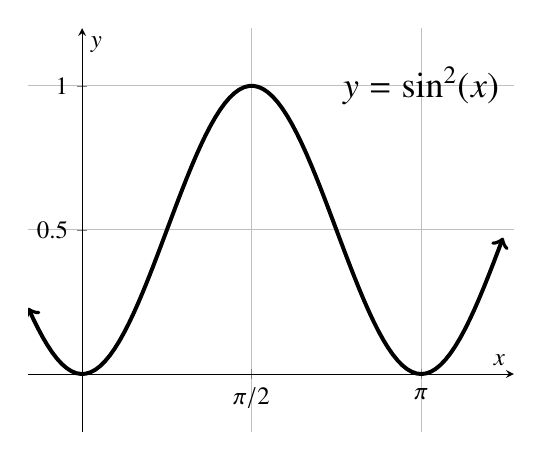
\begin{tikzpicture}[scale = .9]
\begin{axis}[
    axis lines = center,
    xlabel = {$x$},
    ylabel = {$y$},
    xmin = -0.5,
    xmax = 4,
    ymin = -0.2,
    ymax = 1.2,
    samples = 100,
    xtick={0, pi/2, pi}, % Set tick positions
    xticklabels={$0$,  $\pi/2$, $\pi$}, % Label ticks
    xticklabel style={anchor=north}, % Rotate tick labels for better readability
    grid = major]
% Plot the curve
\addplot[<->,ultra thick, black, domain= -.5:3.9] {sin(deg(x))*sin(deg(x))};
\node at (3.14,1){{\Large{$y=\sin^2(x)$}}};
\end{axis}
\end{tikzpicture}
\newpage
%%% TWO
\item (16 points) The region $R$, sketched below, is bounded by $y=\ln(x)$, $x=1$ and $y=1$. \textbf{Set up but do not evaluate} a definite integral to calculate each of the volumes described below. \\
%%Graph of R
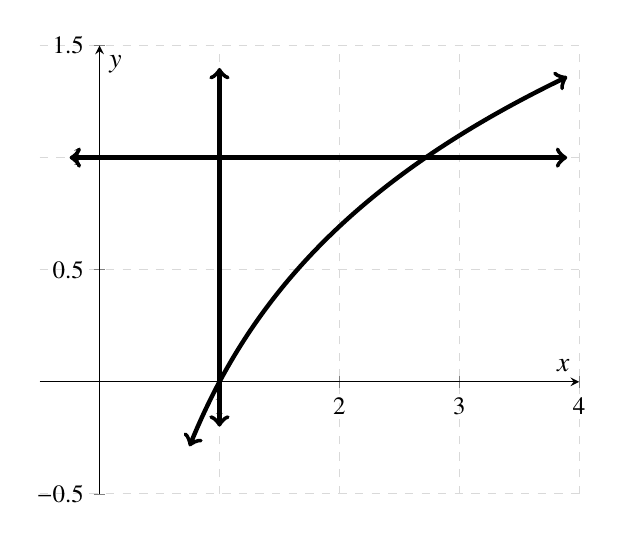
\begin{tikzpicture}
\begin{axis}[
    axis lines = center,
    xlabel = {$x$},
    ylabel = {$y$},
    xmin = -0.5,
    xmax = 4,
    ymin = -0.5,
    ymax = 1.5,
    samples = 100,
    grid = major,
    grid style = {dashed, gray!30},
    tick label style = {font=\small},
]
% Plot the curves
\addplot[<->,ultra thick, black, domain= 0.75:3.9] {ln(x)};
\addplot[<->,ultra thick, black, domain=-0.25:3.9] {1};

% Plot the vertical line x=2
\draw[<->,ultra thick, black] (1,-.2) -- (1,1.4);

\end{axis}
\end{tikzpicture}
	\begin{enumerate}
	\item Use the \textbf{slicing (disks/washers)} method to find the volume generated when $R$ is rotated about the \textbf{${\large{\boldsymbol{x}}}$-axis.} \textit(Set up only.)
	\vfill
	\item Use the \textbf{shell} method to find the volume generated when $R$ is rotated about the \textbf{${\large{\boldsymbol{x}}}$-axis.} \textit(Set up only.)
	\vfill
	\item Use which ever method you prefer to find the volume generated when $R$ is rotated about the \textbf{${\large{\boldsymbol{y}}}$-axis.} \textit(Set up only.) \textbf{State the method you are using.}
	\vfill
	\end{enumerate}
\newpage	

%%%%%%%%%%%
%% Surface Area
%%%%%%%%%%%
%%% THREE
\item (8 points) Set up but do not evaluate integrals to find the surface area of the volume generated when the curve  $y=x^2$ from $x=0$ to $x=3$ is rotated about 
	\begin{enumerate}
	\item the $x$-axis.
	\vfill
	\item the $y$-axis.
	\vfill
	\end{enumerate}	
%%%%%%%%%%%%
%%% DENSITY and Mass: LINEAR
%%%%%%%%%%%%
%%% FOUR
\item (11 points) A 3-meter long whip antenna has linear density $\ds \rho(x) =
  5\ln(x)$ grams per meter for $x$-values in the interval $[1,4].$ Determine
  the mass of the antenna. Include units.  
  
\vfill

\vfill
 \newpage 
  %%%%%%%%%%%%%
 %% WORK , SPRING
 %%%%%%%%%%
 %%%% FIVE
 \item (10 points) 
 	\begin{enumerate}
	\item If 30 Nm of work are required to compress a spring from 5 meters (neutral length) to 4 meters, determine the spring constant $k$ in Hooke's Law.
	\vfill
	\item For the spring in part $a$, how far must the spring be compressed from its natural position if the work required to do so is 120 Nm?\\
 	\vfill
 	\end{enumerate}
 
\newpage
 %%%%%%%%%%%
 %%% Center of Mass
 %%%%%%%%%%%
 %%% SIX
 \item (11 points) Let $R$ be the  region bounded by $y=x^2$ and $y=x$.
	\begin{enumerate}
	\item (3 points) Sketch the region $R.$
	\vfill
	\item (6 points) Set up the definite integrals to compute the center of mass (centroid) $(\bar{x}, \bar{y})$ of $R.$ You do not have to evaluate the integrals.\\
	
	\vspace{.5in}
	
	${\Large{\bar{x}}}= $ \quad \hspace{3in} ${\Large{\bar{y}}}= $\\
	
	\vspace*{-.75in}
	\quad \hspace{1cm}\framebox[60mm]{\rule{0pt}{40mm}} \hspace{1in}\framebox[60mm]{\rule{0pt}{40mm}}
	
	\vfill
	
	\item (2 points) Suppose someone calculates the center of mass of $R$ to be $(\bar{x}, \bar{y}) = (0.8,0.8).$ Is this plausible?  You can and should answer this \textbf{without actually evaluating the integrals in part (b)}.
	
	\vfill
	\end{enumerate}
	
	 \newpage
 
 
 %%%%%%%%%%%%%%%%
 %%% Assortment of Integrals
 %%%%%%%%%%%%%%%%
 %%% SEVEN
 \item (8 points each) Evaluate the indefinite integrals.
 	\begin{enumerate}
	\item  $\ds \int \cos^3(x)\sin^3\left(x\right) \, dx$
	\vfill
	\item  $\displaystyle \int x e^{x/2} \: dx$
	\vfill
	\newpage
 	\item $\ds \int \frac{x+4}{x^2+x-6} \: dx$
	\vfill
	
%	\item $\ds \int \frac{x}{\sqrt{x^2-5}} \: dx$
%	\vfill
	\item $\ds \int \frac{\sqrt{x^2-25}}{x } \: dx$
	\vfill
	\end{enumerate} 
\end{enumerate}
\newpage
%%% EXTRA CREDIT
Extra Credit (5 points) Evaluate the integral $\ds \int x \sin^2 (x) \cos(x) \: dx$\\
\vfill

\hrulefill

\begin{tabular}{ccc}
Half-Angle/Double Angle && Sum and Difference\\
\hline
&&\\
$\sin^2(x)=\frac{1}{2} ( 1-\cos(2x))$&&$\sin(ax)\cos(bx)=\frac{1}{2} ( \sin((a-b)x)+\sin((a+b)x))$\\ &&\\

 $\cos^2(x)=\frac{1}{2} ( 1+\cos(2x))$&&$\sin(ax)\sin(bx)=\frac{1}{2} ( \cos((a-b)x)-\cos((a+b)x))$\\ &&\\
 
$\sin(2x)=2\sin(x)\cos(x)$ &&$\cos(ax)\cos(bx)=\frac{1}{2} ( \cos((a-b)x)+\cos((a+b)x))$\\ &&\\
\end{tabular}
\vspace{0.5in}


$\text{L} = \displaystyle{\int_a^b}\sqrt{1+(f'(x))^2} \: dx$ \hspace{.3in} $\text{S} = \displaystyle{\int_a^b}2 \pi f(x)\sqrt{1+(f'(x))^2} \: dx$

%A conical tank has height = radius = a meters. It is filled with liquid with force density of $k \: N/m^3$. Determine the amount of work needed to pump all the liquid out of the top of the tank.\\
%
%
%Find the mass of a frisbee of radius 6 inch with density function $\rho(x)=e^{-x}$. \textit{A formula in 2.4 that isn't hard, but didn't go over in class... Could give the formula and have a difficult integration, or? Hint: calculate the density in concentric circles?}

\end{document}
